% Options for packages loaded elsewhere
% Options for packages loaded elsewhere
\PassOptionsToPackage{unicode}{hyperref}
\PassOptionsToPackage{hyphens}{url}
%
\documentclass[
  ignorenonframetext,
  aspectratio=169,
  handout]{beamer}
\newif\ifbibliography
\usepackage{pgfpages}
\setbeamertemplate{caption}[numbered]
\setbeamertemplate{caption label separator}{: }
\setbeamercolor{caption name}{fg=normal text.fg}
\beamertemplatenavigationsymbolsempty
% remove section numbering
\setbeamertemplate{part page}{
  \centering
  \begin{beamercolorbox}[sep=16pt,center]{part title}
    \usebeamerfont{part title}\insertpart\par
  \end{beamercolorbox}
}
\setbeamertemplate{section page}{
  \centering
  \begin{beamercolorbox}[sep=12pt,center]{section title}
    \usebeamerfont{section title}\insertsection\par
  \end{beamercolorbox}
}
\setbeamertemplate{subsection page}{
  \centering
  \begin{beamercolorbox}[sep=8pt,center]{subsection title}
    \usebeamerfont{subsection title}\insertsubsection\par
  \end{beamercolorbox}
}
% Prevent slide breaks in the middle of a paragraph
\widowpenalties 1 10000
\raggedbottom
\AtBeginPart{
  \frame{\partpage}
}
\AtBeginSection{
  \ifbibliography
  \else
    \frame{\sectionpage}
  \fi
}
\AtBeginSubsection{
  \frame{\subsectionpage}
}
\usepackage{iftex}
\ifPDFTeX
  \usepackage[T1]{fontenc}
  \usepackage[utf8]{inputenc}
  \usepackage{textcomp} % provide euro and other symbols
\else % if luatex or xetex
  \usepackage{unicode-math} % this also loads fontspec
  \defaultfontfeatures{Scale=MatchLowercase}
  \defaultfontfeatures[\rmfamily]{Ligatures=TeX,Scale=1}
\fi
\usepackage{lmodern}

\ifPDFTeX\else
  % xetex/luatex font selection
\fi
% Use upquote if available, for straight quotes in verbatim environments
\IfFileExists{upquote.sty}{\usepackage{upquote}}{}
\IfFileExists{microtype.sty}{% use microtype if available
  \usepackage[]{microtype}
  \UseMicrotypeSet[protrusion]{basicmath} % disable protrusion for tt fonts
}{}
\makeatletter
\@ifundefined{KOMAClassName}{% if non-KOMA class
  \IfFileExists{parskip.sty}{%
    \usepackage{parskip}
  }{% else
    \setlength{\parindent}{0pt}
    \setlength{\parskip}{6pt plus 2pt minus 1pt}}
}{% if KOMA class
  \KOMAoptions{parskip=half}}
\makeatother


\usepackage{longtable,booktabs,array}
\newcounter{none} % for unnumbered tables
\usepackage{calc} % for calculating minipage widths
\usepackage{caption}
% Make caption package work with longtable
\makeatletter
\def\fnum@table{\tablename~\thetable}
\makeatother
\usepackage{graphicx}
\makeatletter
\newsavebox\pandoc@box
\newcommand*\pandocbounded[1]{% scales image to fit in text height/width
  \sbox\pandoc@box{#1}%
  \Gscale@div\@tempa{\textheight}{\dimexpr\ht\pandoc@box+\dp\pandoc@box\relax}%
  \Gscale@div\@tempb{\linewidth}{\wd\pandoc@box}%
  \ifdim\@tempb\p@<\@tempa\p@\let\@tempa\@tempb\fi% select the smaller of both
  \ifdim\@tempa\p@<\p@\scalebox{\@tempa}{\usebox\pandoc@box}%
  \else\usebox{\pandoc@box}%
  \fi%
}
% Set default figure placement to htbp
\def\fps@figure{htbp}
\makeatother





\setlength{\emergencystretch}{3em} % prevent overfull lines

\providecommand{\tightlist}{%
  \setlength{\itemsep}{0pt}\setlength{\parskip}{0pt}}



 


\makeatletter
\@ifpackageloaded{caption}{}{\usepackage{caption}}
\AtBeginDocument{%
\ifdefined\contentsname
  \renewcommand*\contentsname{Table of contents}
\else
  \newcommand\contentsname{Table of contents}
\fi
\ifdefined\listfigurename
  \renewcommand*\listfigurename{List of Figures}
\else
  \newcommand\listfigurename{List of Figures}
\fi
\ifdefined\listtablename
  \renewcommand*\listtablename{List of Tables}
\else
  \newcommand\listtablename{List of Tables}
\fi
\ifdefined\figurename
  \renewcommand*\figurename{Figure}
\else
  \newcommand\figurename{Figure}
\fi
\ifdefined\tablename
  \renewcommand*\tablename{Table}
\else
  \newcommand\tablename{Table}
\fi
}
\@ifpackageloaded{float}{}{\usepackage{float}}
\floatstyle{ruled}
\@ifundefined{c@chapter}{\newfloat{codelisting}{h}{lop}}{\newfloat{codelisting}{h}{lop}[chapter]}
\floatname{codelisting}{Listing}
\newcommand*\listoflistings{\listof{codelisting}{List of Listings}}
\makeatother
\makeatletter
\makeatother
\makeatletter
\@ifpackageloaded{caption}{}{\usepackage{caption}}
\@ifpackageloaded{subcaption}{}{\usepackage{subcaption}}
\makeatother

\usepackage{bookmark}
\IfFileExists{xurl.sty}{\usepackage{xurl}}{} % add URL line breaks if available
\urlstyle{same}
\hypersetup{
  pdftitle={Characteristics of Quantum Wavefunctions},
  pdfauthor={Davit Potoyan},
  hidelinks,
  pdfcreator={LaTeX via pandoc}}


\title{\texorpdfstring{Characteristics of Quantum
Wavefunctions}{Characteristics of Quantum Wavefunctions}}
\subtitle{\texorpdfstring{Chem 3240 · Lecture
3.5}{Chem 3240 · Lecture 3.5}}
\author{Davit Potoyan}
\date{}

\begin{document}
\frame{\titlepage}


\begin{frame}
\begin{block}{Quantum objects go where classical ones cannot}
\protect\phantomsection\label{quantum-objects-go-where-classical-ones-cannot}
\begin{columns}[T]
\begin{column}{0.55\linewidth}
\pandocbounded{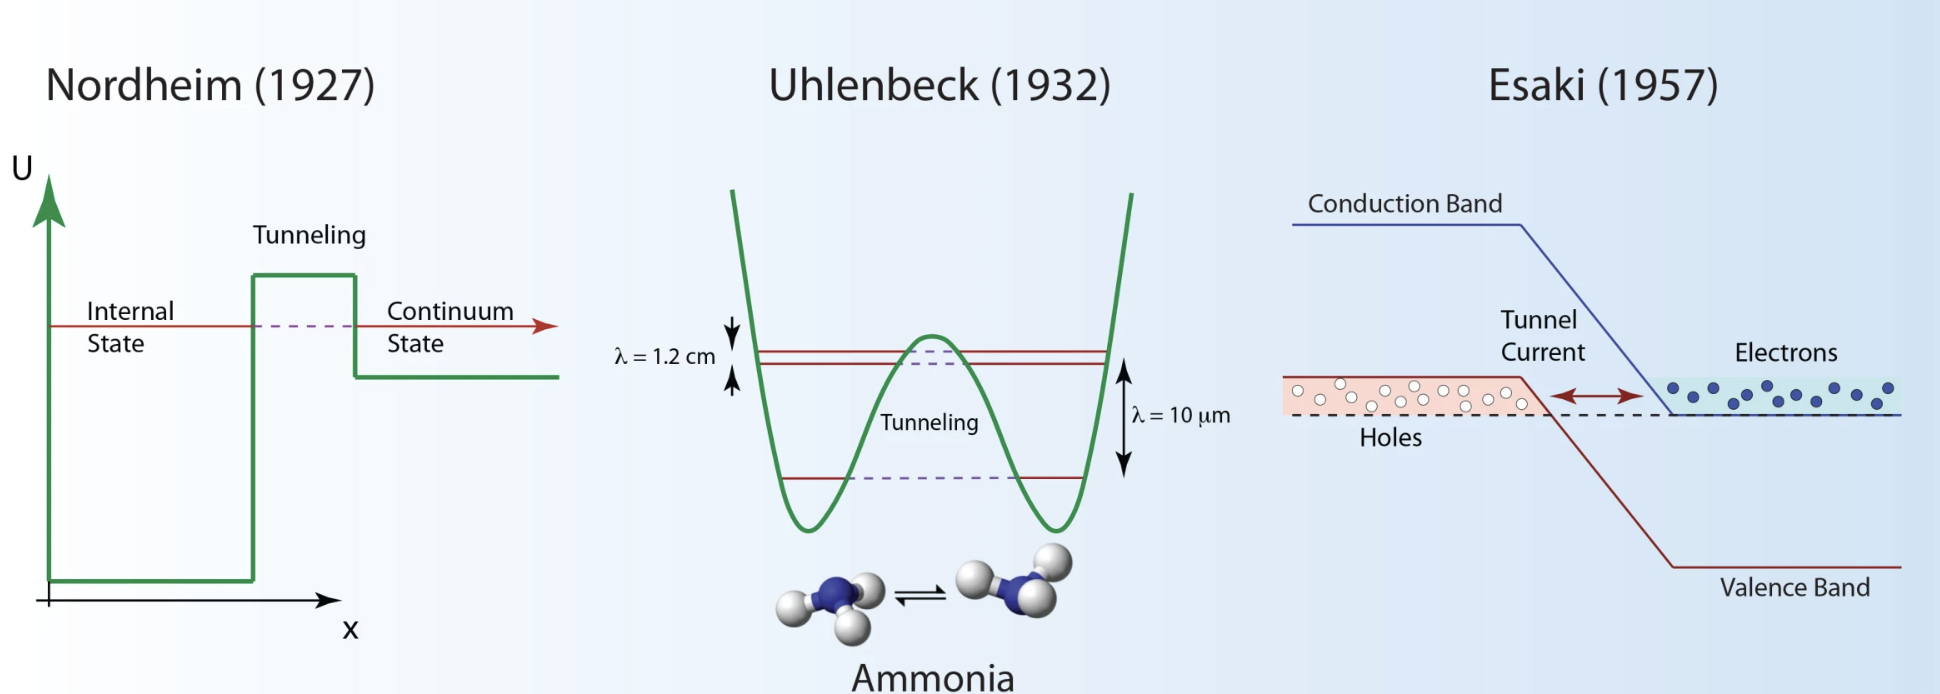
\includegraphics[keepaspectratio]{../../ch03/images/tunnel1.png}}
\end{column}

\begin{column}{0.45\linewidth}
\begin{itemize}
\tightlist
\item
  \textbf{Tunneling} into classically forbidden regions
\end{itemize}

\begin{itemize}
\tightlist
\item
  Electron emission, \textbf{ammonia inversion}, tunnel diodes
\end{itemize}

\begin{itemize}
\tightlist
\item
  The \textbf{finite well} is the realistic model that allows it
\end{itemize}
\end{column}
\end{columns}
\end{block}

\begin{block}{Reading a wavefunction qualitatively}
\protect\phantomsection\label{reading-a-wavefunction-qualitatively}
\begin{columns}[T]
\begin{column}{0.5\linewidth}
\pandocbounded{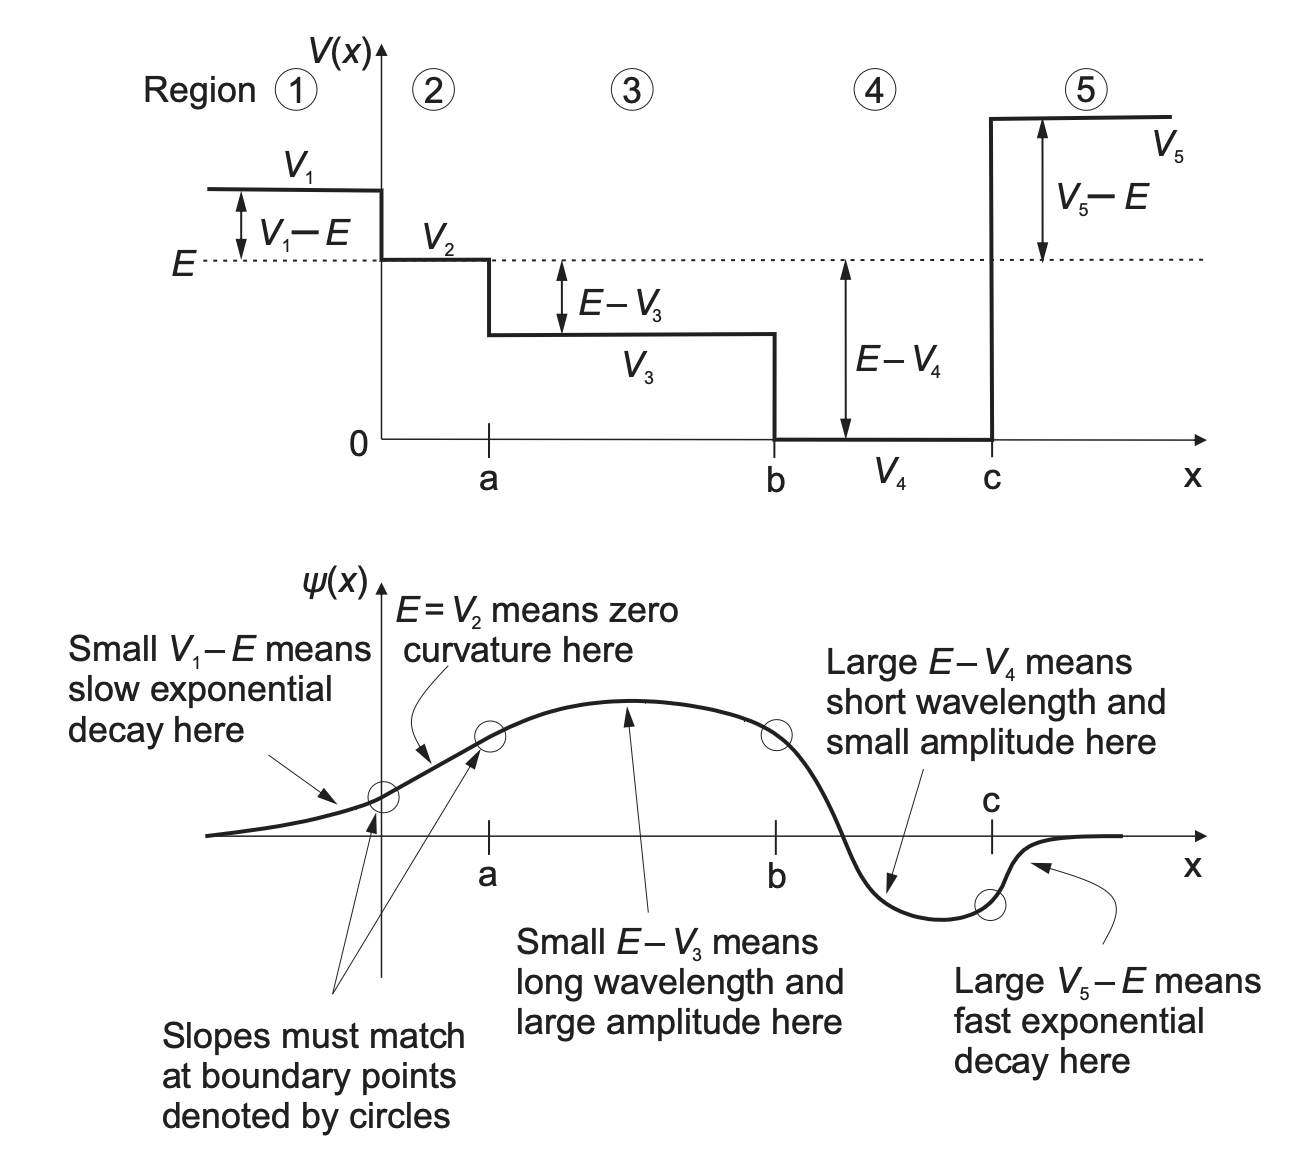
\includegraphics[keepaspectratio]{../../ch03/images/gen_psi1.png}}
\end{column}

\begin{column}{0.5\linewidth}
\begin{itemize}
\tightlist
\item
  \textbf{Curvature} is set by the sign of \(E - V\)
\end{itemize}

\begin{itemize}
\tightlist
\item
  \(E > V\): \(\psi\) \textbf{oscillates}, curves toward axis
\end{itemize}

\begin{itemize}
\tightlist
\item
  \(E < V\): \(\psi\) \textbf{decays}, curves away from axis
\end{itemize}
\end{column}
\end{columns}
\end{block}

\begin{block}{Curvature follows the potential}
\protect\phantomsection\label{curvature-follows-the-potential}
\begin{columns}[T]
\begin{column}{0.5\linewidth}
\pandocbounded{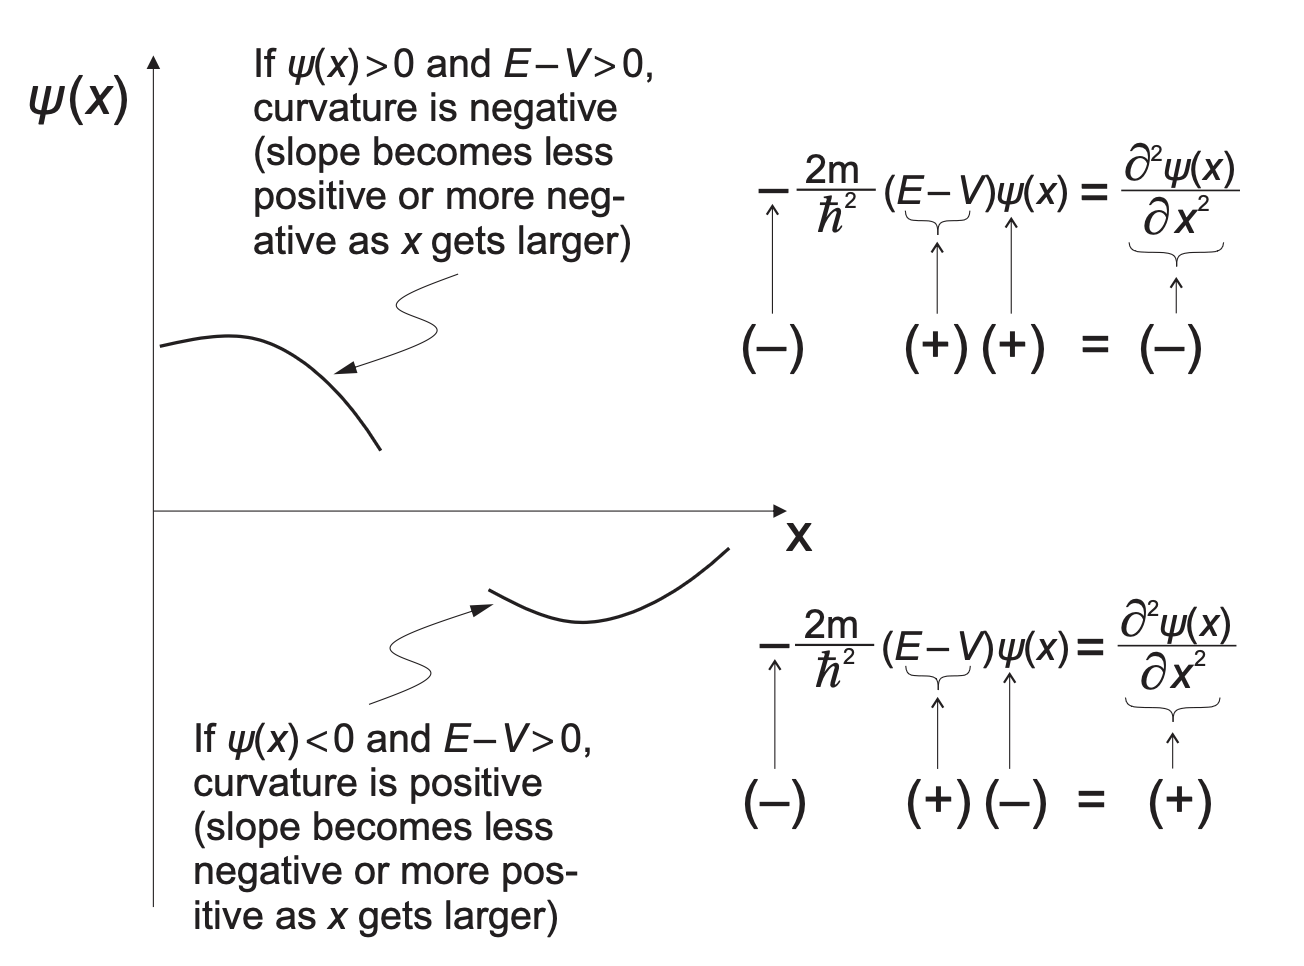
\includegraphics[keepaspectratio]{../../ch03/images/gen_psi2.png}}
\end{column}

\begin{column}{0.5\linewidth}
\begin{itemize}
\tightlist
\item
  A \textbf{stepped potential} changes the local wavelength
\end{itemize}

\begin{itemize}
\tightlist
\item
  Higher kinetic energy means \textbf{shorter wavelength}
\end{itemize}

\begin{itemize}
\tightlist
\item
  \(\psi\) stays smooth and continuous everywhere
\end{itemize}
\end{column}
\end{columns}
\end{block}

\begin{block}{Three regions, three solutions}
\protect\phantomsection\label{three-regions-three-solutions}
The finite square well: \(V=0\) inside, \(V=V_0\) outside.

\[
-\frac{\hbar^2}{2m}\frac{d^2\psi(x)}{d{x}^2}+V(x)\psi(x) =E\psi(x)
\]

\[
\text{Region I:  }  V(x) = V_0 ~~~~~~~~~~~~~~~~ x \leq-\frac{L}{2} ~~~~~ \psi_{I} = A e^{\beta  x} \\
\text{Region II: }  V(x) = 0 ~~~ -\frac{L}{2} \leq x \leq\frac{L}{2} ~~~~~~~ \psi_{II} = B \cos(k x) + C \sin(k x)\\
\text{Region III:}  V(x) = V_0 ~~~~~~~~~~~~~~  x \geq \frac{L}{2}  ~~~~~~~ \psi_{III} = D e^{-\beta x}
\]
\end{block}

\begin{block}{Inside vs outside the well}
\protect\phantomsection\label{inside-vs-outside-the-well}
\begin{columns}[T]
\begin{column}{0.5\linewidth}
\textbf{Inside} (\(E > V\)) \[
\psi(x)=A\sin(kx)+B\cos(kx)
\] ::: \{.fragment\} Oscillatory.
\end{column}
\end{columns}

\begin{column}{0.5\linewidth}
\textbf{Outside} (\(E < V_0\)) ::: \{.fragment\} \[
k^2 = \frac{2m(V_0 - E)}{\hbar^2}
\]
\end{column}

Real \(\beta\): \textbf{exponential decay}, an evanescent wave.

:::

::::
\end{block}

\begin{block}{Why continuity matters}
\protect\phantomsection\label{why-continuity-matters}
\begin{columns}[T]
\begin{column}{0.5\linewidth}
\pandocbounded{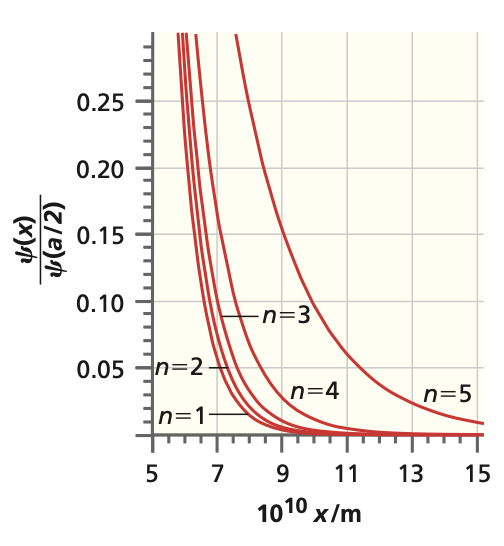
\includegraphics[keepaspectratio]{../../ch03/images/decay_psi.png}}
\end{column}

\begin{column}{0.5\linewidth}
\begin{itemize}
\tightlist
\item
  Match \(\psi\) \textbf{and} \(\psi'\) at each boundary
\end{itemize}

\[
\psi_{I}\!\left(-\tfrac{L}{2}\right) = \psi_{II}\!\left(-\tfrac{L}{2}\right)
\]

\begin{itemize}
\tightlist
\item
  \(\psi'\) continuous so \(\psi''\) exists
\end{itemize}

\begin{itemize}
\tightlist
\item
  \(\psi''\) is the \textbf{kinetic energy} operator: must be defined
\end{itemize}
\end{column}
\end{columns}
\end{block}

\begin{block}{Even and odd solutions}
\protect\phantomsection\label{even-and-odd-solutions}
The well is \textbf{symmetric} about \(x=0\), so states split by parity.

\begin{columns}[T]
\begin{column}{0.5\linewidth}
\textbf{Even} (\(\psi(x)=\psi(-x)\)) \[
\psi_{II}(x) = B \cos(k x)
\] \[
\beta = k\tan\left(k\frac{L}{2}\right)
\]
\end{column}

\begin{column}{0.5\linewidth}
\textbf{Odd} (\(\psi(x)=-\psi(-x)\)) \[
\psi_{II}(x) = C \sin(k x)
\] \[
\beta = -\frac{k}{\tan\left(k\frac{L}{2}\right)}
\]
\end{column}
\end{columns}

No closed form: solve \textbf{graphically or numerically}.
\end{block}

\begin{block}{Wavefunctions leak out}
\protect\phantomsection\label{wavefunctions-leak-out}
\begin{columns}[T]
\begin{column}{0.55\linewidth}
\pandocbounded{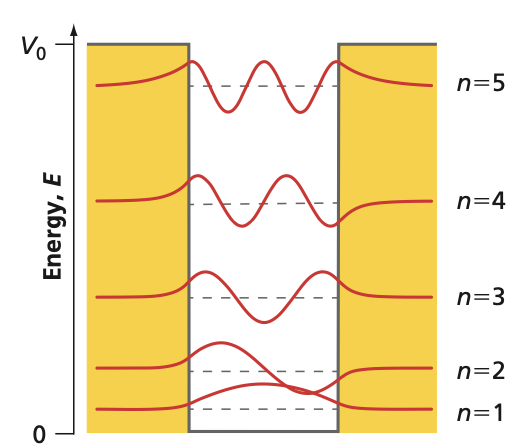
\includegraphics[keepaspectratio]{../../ch03/images/fin_pib.png}}
\end{column}

\begin{column}{0.45\linewidth}
\begin{itemize}
\tightlist
\item
  \(\psi\) extends into the \textbf{classically forbidden} region
\end{itemize}

\begin{itemize}
\tightlist
\item
  Green area: probability of being \textbf{outside} the well
\end{itemize}

\begin{itemize}
\tightlist
\item
  Leakage \textbf{grows} as \(V_0 - E \to 0\)
\end{itemize}
\end{column}
\end{columns}
\end{block}

\begin{block}{Tunneling probability}
\protect\phantomsection\label{tunneling-probability}
The chance of finding the particle outside the box:

\[
P\left(-\frac{L}{2}>x>\frac{L}{2}\right)=\frac{\int^{\frac{-L}{2}}_{-\infty} |\psi(x)|^2\ dx +\int^{+\infty}_{\frac{L}{2}} |\psi(x)|^2\ dx }{\int_{-\infty}^{+\infty} |\psi(x)|^2\ dx }
\]

\begin{itemize}
\tightlist
\item
  States \textbf{near the top} of the well tunnel most
\end{itemize}
\end{block}

\begin{block}{Finite vs infinite well}
\protect\phantomsection\label{finite-vs-infinite-well}
\begin{itemize}
\tightlist
\item
  Finite well has a \textbf{finite number} of bound states
\end{itemize}

\begin{itemize}
\tightlist
\item
  Low states: energies nearly \textbf{match} the infinite well
\end{itemize}

\begin{itemize}
\tightlist
\item
  High states: \(\psi\) spreads out, \textbf{longer wavelength}
\end{itemize}

\begin{itemize}
\tightlist
\item
  Longer wavelength means smaller \(k\), so \textbf{lower energy}
\end{itemize}
\end{block}
\end{frame}

\begin{frame}{Takeaway}
\protect\phantomsection\label{takeaway}
\begin{quote}
Wavefunctions stay smooth, curving and decaying according to \(E - V\),
and they leak into forbidden regions, giving the finite well its
tunneling and its limited set of bound states.
\end{quote}
\end{frame}




\end{document}
